% Created by tikzDevice version 0.10.1 on 2020-02-15 16:17:50
% !TEX encoding = UTF-8 Unicode
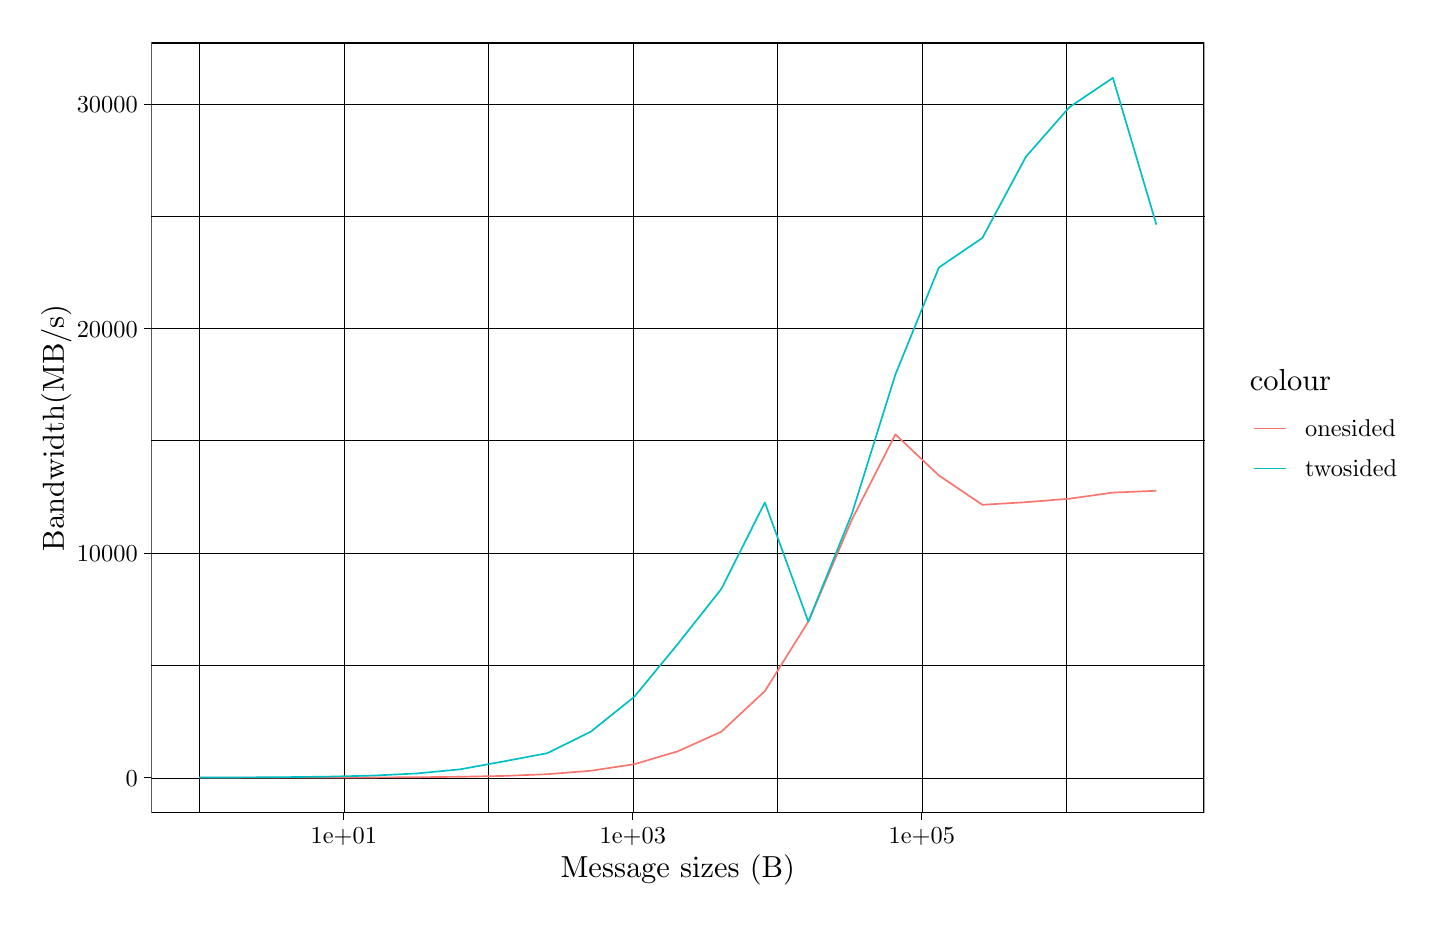
\begin{tikzpicture}[x=1pt,y=1pt]
\definecolor{fillColor}{RGB}{255,255,255}
\path[use as bounding box,fill=fillColor,fill opacity=0.00] (0,0) rectangle (505.89,314.37);
\begin{scope}
\path[clip] (  0.00,  0.00) rectangle (505.89,314.37);
\definecolor{drawColor}{RGB}{255,255,255}
\definecolor{fillColor}{RGB}{255,255,255}

\path[draw=drawColor,line width= 0.6pt,line join=round,line cap=round,fill=fillColor] (  0.00,  0.00) rectangle (505.89,314.37);
\end{scope}
\begin{scope}
\path[clip] ( 44.71, 30.72) rectangle (425.15,308.87);
\definecolor{fillColor}{RGB}{255,255,255}

\path[fill=fillColor] ( 44.71, 30.72) rectangle (425.15,308.87);
\definecolor{drawColor}{RGB}{0,0,0}

\path[draw=drawColor,line width= 0.0pt,line join=round] ( 44.71, 83.93) --
	(425.15, 83.93);

\path[draw=drawColor,line width= 0.0pt,line join=round] ( 44.71,165.05) --
	(425.15,165.05);

\path[draw=drawColor,line width= 0.0pt,line join=round] ( 44.71,246.18) --
	(425.15,246.18);

\path[draw=drawColor,line width= 0.0pt,line join=round] ( 62.01, 30.72) --
	( 62.01,308.87);

\path[draw=drawColor,line width= 0.0pt,line join=round] (166.45, 30.72) --
	(166.45,308.87);

\path[draw=drawColor,line width= 0.0pt,line join=round] (270.90, 30.72) --
	(270.90,308.87);

\path[draw=drawColor,line width= 0.0pt,line join=round] (375.34, 30.72) --
	(375.34,308.87);

\path[draw=drawColor,line width= 0.1pt,line join=round] ( 44.71, 43.36) --
	(425.15, 43.36);

\path[draw=drawColor,line width= 0.1pt,line join=round] ( 44.71,124.49) --
	(425.15,124.49);

\path[draw=drawColor,line width= 0.1pt,line join=round] ( 44.71,205.62) --
	(425.15,205.62);

\path[draw=drawColor,line width= 0.1pt,line join=round] ( 44.71,286.74) --
	(425.15,286.74);

\path[draw=drawColor,line width= 0.1pt,line join=round] (114.23, 30.72) --
	(114.23,308.87);

\path[draw=drawColor,line width= 0.1pt,line join=round] (218.67, 30.72) --
	(218.67,308.87);

\path[draw=drawColor,line width= 0.1pt,line join=round] (323.12, 30.72) --
	(323.12,308.87);
\definecolor{drawColor}{RGB}{248,118,109}

\path[draw=drawColor,line width= 0.6pt,line join=round] ( 62.01, 43.37) --
	( 77.73, 43.37) --
	( 93.45, 43.38) --
	(109.17, 43.40) --
	(124.89, 43.44) --
	(140.61, 43.52) --
	(156.33, 43.68) --
	(172.05, 43.99) --
	(187.77, 44.62) --
	(203.49, 45.86) --
	(219.21, 48.23) --
	(234.93, 52.89) --
	(250.65, 59.97) --
	(266.37, 74.62) --
	(282.09, 99.76) --
	(297.81,136.55) --
	(313.54,167.41) --
	(329.26,152.56) --
	(344.98,141.96) --
	(360.70,142.90) --
	(376.42,144.17) --
	(392.14,146.37) --
	(407.86,147.03);
\definecolor{drawColor}{RGB}{0,191,196}

\path[draw=drawColor,line width= 0.6pt,line join=round] ( 62.01, 43.41) --
	( 77.73, 43.45) --
	( 93.45, 43.55) --
	(109.17, 43.74) --
	(124.89, 44.12) --
	(140.61, 44.88) --
	(156.33, 46.38) --
	(172.05, 49.24) --
	(187.77, 52.21) --
	(203.49, 59.98) --
	(219.21, 72.60) --
	(234.93, 91.67) --
	(250.65,111.55) --
	(266.37,142.79) --
	(282.09, 99.74) --
	(297.81,138.67) --
	(313.54,189.01) --
	(329.26,227.70) --
	(344.98,238.38) --
	(360.70,267.72) --
	(376.42,285.64) --
	(392.14,296.23) --
	(407.86,243.17);
\definecolor{drawColor}{RGB}{0,0,0}

\path[draw=drawColor,line width= 0.6pt,line join=round,line cap=round] ( 44.71, 30.72) rectangle (425.15,308.87);
\end{scope}
\begin{scope}
\path[clip] (  0.00,  0.00) rectangle (505.89,314.37);
\definecolor{drawColor}{RGB}{0,0,0}

\node[text=drawColor,anchor=base east,inner sep=0pt, outer sep=0pt, scale=  0.88] at ( 39.76, 40.33) {0};

\node[text=drawColor,anchor=base east,inner sep=0pt, outer sep=0pt, scale=  0.88] at ( 39.76,121.46) {10000};

\node[text=drawColor,anchor=base east,inner sep=0pt, outer sep=0pt, scale=  0.88] at ( 39.76,202.58) {20000};

\node[text=drawColor,anchor=base east,inner sep=0pt, outer sep=0pt, scale=  0.88] at ( 39.76,283.71) {30000};
\end{scope}
\begin{scope}
\path[clip] (  0.00,  0.00) rectangle (505.89,314.37);
\definecolor{drawColor}{RGB}{0,0,0}

\path[draw=drawColor,line width= 0.3pt,line join=round] ( 41.96, 43.36) --
	( 44.71, 43.36);

\path[draw=drawColor,line width= 0.3pt,line join=round] ( 41.96,124.49) --
	( 44.71,124.49);

\path[draw=drawColor,line width= 0.3pt,line join=round] ( 41.96,205.62) --
	( 44.71,205.62);

\path[draw=drawColor,line width= 0.3pt,line join=round] ( 41.96,286.74) --
	( 44.71,286.74);
\end{scope}
\begin{scope}
\path[clip] (  0.00,  0.00) rectangle (505.89,314.37);
\definecolor{drawColor}{RGB}{0,0,0}

\path[draw=drawColor,line width= 0.3pt,line join=round] (114.23, 27.97) --
	(114.23, 30.72);

\path[draw=drawColor,line width= 0.3pt,line join=round] (218.67, 27.97) --
	(218.67, 30.72);

\path[draw=drawColor,line width= 0.3pt,line join=round] (323.12, 27.97) --
	(323.12, 30.72);
\end{scope}
\begin{scope}
\path[clip] (  0.00,  0.00) rectangle (505.89,314.37);
\definecolor{drawColor}{RGB}{0,0,0}

\node[text=drawColor,anchor=base,inner sep=0pt, outer sep=0pt, scale=  0.88] at (114.23, 19.71) {1e+01};

\node[text=drawColor,anchor=base,inner sep=0pt, outer sep=0pt, scale=  0.88] at (218.67, 19.71) {1e+03};

\node[text=drawColor,anchor=base,inner sep=0pt, outer sep=0pt, scale=  0.88] at (323.12, 19.71) {1e+05};
\end{scope}
\begin{scope}
\path[clip] (  0.00,  0.00) rectangle (505.89,314.37);
\definecolor{drawColor}{RGB}{0,0,0}

\node[text=drawColor,anchor=base,inner sep=0pt, outer sep=0pt, scale=  1.10] at (234.93,  7.44) {Message sizes (B)};
\end{scope}
\begin{scope}
\path[clip] (  0.00,  0.00) rectangle (505.89,314.37);
\definecolor{drawColor}{RGB}{0,0,0}

\node[text=drawColor,rotate= 90.00,anchor=base,inner sep=0pt, outer sep=0pt, scale=  1.10] at ( 13.08,169.80) {Bandwidth(MB/s)};
\end{scope}
\begin{scope}
\path[clip] (  0.00,  0.00) rectangle (505.89,314.37);
\definecolor{fillColor}{RGB}{255,255,255}

\path[fill=fillColor] (436.15,142.34) rectangle (500.39,197.26);
\end{scope}
\begin{scope}
\path[clip] (  0.00,  0.00) rectangle (505.89,314.37);
\definecolor{drawColor}{RGB}{0,0,0}

\node[text=drawColor,anchor=base west,inner sep=0pt, outer sep=0pt, scale=  1.10] at (441.65,183.22) {colour};
\end{scope}
\begin{scope}
\path[clip] (  0.00,  0.00) rectangle (505.89,314.37);
\definecolor{fillColor}{RGB}{255,255,255}

\path[fill=fillColor] (441.65,162.29) rectangle (456.10,176.74);
\end{scope}
\begin{scope}
\path[clip] (  0.00,  0.00) rectangle (505.89,314.37);
\definecolor{drawColor}{RGB}{248,118,109}

\path[draw=drawColor,line width= 0.6pt,line join=round] (443.10,169.52) -- (454.66,169.52);
\end{scope}
\begin{scope}
\path[clip] (  0.00,  0.00) rectangle (505.89,314.37);
\definecolor{drawColor}{RGB}{248,118,109}

\path[draw=drawColor,line width= 0.6pt,line join=round] (443.10,169.52) -- (454.66,169.52);
\end{scope}
\begin{scope}
\path[clip] (  0.00,  0.00) rectangle (505.89,314.37);
\definecolor{fillColor}{RGB}{255,255,255}

\path[fill=fillColor] (441.65,147.84) rectangle (456.10,162.29);
\end{scope}
\begin{scope}
\path[clip] (  0.00,  0.00) rectangle (505.89,314.37);
\definecolor{drawColor}{RGB}{0,191,196}

\path[draw=drawColor,line width= 0.6pt,line join=round] (443.10,155.06) -- (454.66,155.06);
\end{scope}
\begin{scope}
\path[clip] (  0.00,  0.00) rectangle (505.89,314.37);
\definecolor{drawColor}{RGB}{0,191,196}

\path[draw=drawColor,line width= 0.6pt,line join=round] (443.10,155.06) -- (454.66,155.06);
\end{scope}
\begin{scope}
\path[clip] (  0.00,  0.00) rectangle (505.89,314.37);
\definecolor{drawColor}{RGB}{0,0,0}

\node[text=drawColor,anchor=base west,inner sep=0pt, outer sep=0pt, scale=  0.88] at (461.60,166.49) {onesided};
\end{scope}
\begin{scope}
\path[clip] (  0.00,  0.00) rectangle (505.89,314.37);
\definecolor{drawColor}{RGB}{0,0,0}

\node[text=drawColor,anchor=base west,inner sep=0pt, outer sep=0pt, scale=  0.88] at (461.60,152.03) {twosided};
\end{scope}
\end{tikzpicture}
